\documentclass[11pt,a4paper]{article}

% ---------------------------------------------------------------- fill these in
\newcommand{\studentname}{Anas Tamer}
\newcommand{\studentid}{22u0005}
% -----------------------------------------------------------------------------

\usepackage[margin=2.3cm]{geometry}
\usepackage[T1]{fontenc}
\usepackage{lmodern}
\usepackage{amsmath,amssymb}
\usepackage{graphicx}
\usepackage{booktabs}
\usepackage{xcolor}
\usepackage{listings}
\usepackage{float}
\usepackage{tikz}
\usetikzlibrary{positioning,arrows.meta}
\usepackage[hidelinks]{hyperref}
\setlength{\emergencystretch}{3em}  % let long \texttt words wrap without overflowing

\definecolor{codebg}{RGB}{247,247,247}
\definecolor{kw}{RGB}{0,0,160}
\definecolor{cm}{RGB}{0,120,0}
\definecolor{st}{RGB}{160,40,0}
\lstset{
  language=Python, basicstyle=\ttfamily\small, backgroundcolor=\color{codebg},
  keywordstyle=\color{kw}\bfseries, commentstyle=\color{cm}\itshape, stringstyle=\color{st},
  frame=single, rulecolor=\color{gray!40}, breaklines=true, showstringspaces=false,
  columns=fullflexible, keepspaces=true, xleftmargin=4pt, xrightmargin=4pt
}

\begin{document}

% ================================================================== title page
\begin{titlepage}
\centering
{\large\textbf{AIN SHAMS UNIVERSITY}\par}
{\large\textbf{FACULTY OF ENGINEERING}\par}
{i-CREDIT HOURS ENGINEERING PROGRAMS\par}
{\itshape Computer Engineering and Software Systems\par}
\vspace{3cm}
{\Large CSE485--CSE488: Deep Learning\par}
\vspace{0.6cm}
{\LARGE\bfseries Assignment 1: MicroGrad\par}
{\Large A Scalar Automatic Differentiation Engine\par}
\vspace{0.6cm}
{\large Documentation Report\par}
\vfill
{\large \studentname\par}
{\large Student ID: \studentid\par}
\vspace{1cm}
{\large \today\par}
\end{titlepage}

\tableofcontents
\newpage

% ================================================================== 1
\section{Introduction}
Modern deep-learning frameworks compute gradients automatically. This assignment builds that machinery
from scratch at the smallest possible scale: every scalar is an object that remembers how it was
produced, and gradients are obtained by applying the chain rule backwards through the resulting graph.
The design follows Andrej Karpathy's \texttt{micrograd}.

The implementation consists of two files of the provided template:
\begin{itemize}
  \item \texttt{src/engine.py}: the \texttt{Value} class (graph construction, local derivatives,
        topological sort, backpropagation);
  \item \texttt{src/nn.py}: \texttt{Neuron}, \texttt{Layer} and \texttt{MLP}, built only from \texttt{Value} objects.
\end{itemize}
No PyTorch, TensorFlow or JAX is used. The demo notebook uses NumPy, scikit-learn and Matplotlib only to
generate data and draw plots.

% ================================================================== 2
\section{Assignment Objectives}
Following the assignment specification:
\begin{enumerate}
  \item Implement \texttt{Value} to store scalar data and gradients.
  \item Overload \texttt{\_\_add\_\_}, \texttt{\_\_mul\_\_}, \texttt{\_\_pow\_\_} (and the derived operators) to build the forward graph.
  \item Implement local derivatives (\texttt{\_backward}) for every operator and for \texttt{tanh} and \texttt{exp}.
  \item Implement the global \texttt{backward()} using a topological sort.
  \item Implement \texttt{Neuron}, \texttt{Layer} and \texttt{MLP} with random initialisation and forward passes.
\end{enumerate}

% ================================================================== 3
\section{System Architecture}
\begin{figure}[H]
\centering
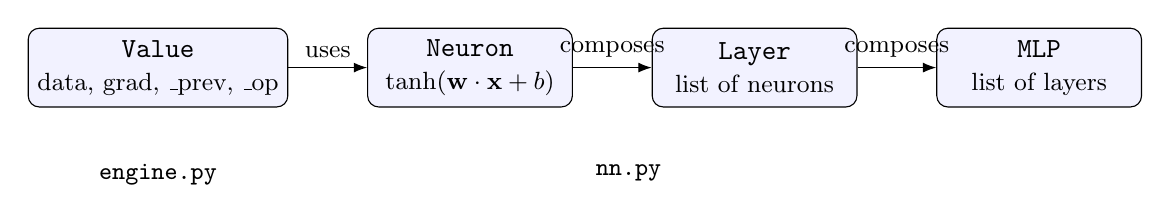
\begin{tikzpicture}[node distance=1.0cm and 1.0cm, box/.style={draw, rounded corners, align=center, minimum width=2.6cm, minimum height=1.0cm, fill=blue!5}]
  \node[box] (val) {\texttt{Value}\\\small data, grad, \_prev, \_op};
  \node[box, right=of val] (neu) {\texttt{Neuron}\\\small $\tanh(\mathbf{w}\cdot\mathbf{x}+b)$};
  \node[box, right=of neu] (lay) {\texttt{Layer}\\\small list of neurons};
  \node[box, right=of lay] (mlp) {\texttt{MLP}\\\small list of layers};
  \draw[-{Latex}] (val) -- node[above]{\small uses} (neu);
  \draw[-{Latex}] (neu) -- node[above]{\small composes} (lay);
  \draw[-{Latex}] (lay) -- node[above]{\small composes} (mlp);
  \node[below=0.6cm of val, align=center] {\small\texttt{engine.py}};
  \node[below=0.6cm of lay, align=center, xshift=-1.6cm] {\small\texttt{nn.py}};
\end{tikzpicture}
\caption{The two-layer architecture: the autodiff engine and the network API built on top of it.}
\end{figure}
The network classes never compute gradients themselves. They only create \texttt{Value} parameters and
combine them with ordinary Python operators, and the engine does the rest. Each class exposes
\texttt{parameters()} (a flat list of \texttt{Value} objects) and \texttt{zero\_grad()}.

% ================================================================== 4
\section{The Computational Graph}
A computation such as $L = (a\cdot b + c)\cdot f$ is represented as a directed acyclic graph (DAG). Leaves
are inputs or parameters, internal nodes are results of operations, and edges point from an operand to the
result. Figure~\ref{fig:graph} shows this graph as produced by our engine (drawn in the notebook from
\texttt{\_get\_topo()}) \emph{after} calling \texttt{L.backward()}.
\begin{figure}[H]
\centering
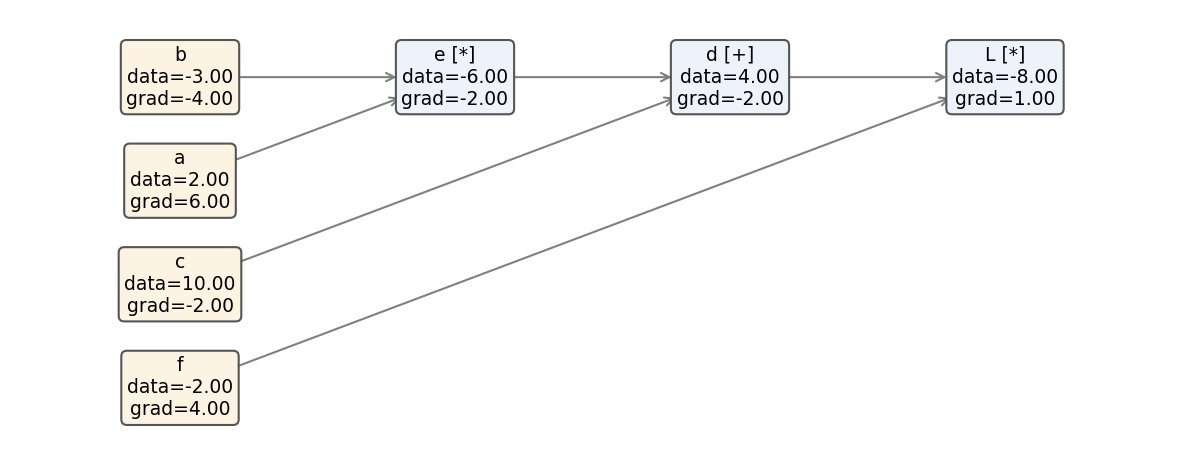
\includegraphics[width=0.95\linewidth]{figures/graph_backward.png}
\caption{Graph for $L=(ab+c)f$ with $a=2,b=-3,c=10,f=-2$: forward values and the gradients from backprop.}
\label{fig:graph}
\end{figure}

% ================================================================== 5
\section{Value Class Design}
\begin{lstlisting}
class Value:
    def __init__(self, data, _children=(), _op='', label=''):
        self.data = data                 # scalar forward value
        self.grad = 0.0                  # dL/d(self), filled by backward()
        self._backward = lambda: None    # local chain-rule step (leaves: no-op)
        self._prev = set(_children)      # operands this node was computed from
        self._op = _op                   # operation label, e.g. '+', '*', 'tanh'
        self.label = label
\end{lstlisting}
\begin{itemize}
  \item \texttt{\_prev} is a \emph{set}, so \texttt{a + a} stores \texttt{a} once. The gradient is still
        counted twice because the closure of the addition adds to \texttt{self.grad} and \texttt{other.grad}, which are the same object.
  \item \texttt{\_backward} is a closure created inside each operator. It captures the operands and the
        output node, so it can apply the local derivative later without storing extra state.
  \item \texttt{\_\_repr\_\_} returns \texttt{Value(data=...)}. \texttt{\_\_int\_\_}/\texttt{\_\_float\_\_}
        convert the stored data. \texttt{reset\_grad()} sets \texttt{grad} back to $0$.
\end{itemize}

% ================================================================== 6
\section{Operator Overloading}
Every operator returns a new \texttt{Value} whose \texttt{\_prev} contains its operands. Plain numbers are
wrapped into constant \texttt{Value}s by a small helper. Any other type makes the operator return
\texttt{NotImplemented}, which Python turns into a \texttt{TypeError} (e.g.\ \texttt{Value(2.0) + "string"}):
\begin{lstlisting}
@staticmethod
def _wrap(other):
    if isinstance(other, Value):
        return other
    if isinstance(other, (int, float)):
        return Value(other)
    return None          # caller returns NotImplemented -> TypeError

def __add__(self, other):
    other = Value._wrap(other)
    if other is None:
        return NotImplemented
    out = Value(self.data + other.data, (self, other), '+')
    def _backward():
        self.grad += 1.0 * out.grad
        other.grad += 1.0 * out.grad
    out._backward = _backward
    return out
\end{lstlisting}
Only $+$, $\times$, power, $\tanh$ and $\exp$ have their own backward rules. The other operators are
\emph{compositions}, so their gradients come out of the chain rule automatically:
\begin{center}
\begin{tabular}{ll}
\toprule
Operator & Implementation \\
\midrule
\texttt{-a} (\texttt{\_\_neg\_\_}) & \texttt{a * -1} \\
\texttt{a - b} (\texttt{\_\_sub\_\_}) & \texttt{a + (-b)} \\
\texttt{a / b} (\texttt{\_\_truediv\_\_}) & \texttt{a * b**-1} \\
\texttt{2 + a}, \texttt{2 * a}, \texttt{2 - a}, \texttt{2 / a} & \texttt{\_\_radd\_\_}, \texttt{\_\_rmul\_\_}, \texttt{\_\_rsub\_\_}, \texttt{\_\_rtruediv\_\_} \\
\bottomrule
\end{tabular}
\end{center}
Division by zero raises \texttt{ZeroDivisionError} naturally, because $0^{-1}$ is evaluated by Python
during the forward pass of \texttt{b**-1}. The exponent of \texttt{\_\_pow\_\_} must be an \texttt{int}
or \texttt{float} (enforced with \texttt{assert}). A \texttt{Value} exponent is not supported.

% ================================================================== 7
\section{Mathematical Derivations: Local Derivatives}
Let $L$ be the final scalar output and write $\bar{v} = \partial L/\partial v$ for the gradient stored in
\texttt{v.grad}. Each \texttt{\_backward} receives $\bar{o}$ of its output $o$ and adds
$\bar{o}\cdot \partial o/\partial x$ to each input $x$.

\paragraph{Addition} $o = a + b$:
\[
\frac{\partial o}{\partial a} = 1,\quad \frac{\partial o}{\partial b} = 1
\;\Longrightarrow\; \bar a \mathrel{+}= \bar o,\; \bar b \mathrel{+}= \bar o .
\]
\paragraph{Multiplication} $o = a\,b$:
\[
\frac{\partial o}{\partial a} = b,\quad \frac{\partial o}{\partial b} = a
\;\Longrightarrow\; \bar a \mathrel{+}= b\,\bar o,\; \bar b \mathrel{+}= a\,\bar o .
\]
\paragraph{Power} $o = a^n$, $n$ a constant:
\[
\frac{\partial o}{\partial a} = n\,a^{n-1} \;\Longrightarrow\; \bar a \mathrel{+}= n\,a^{n-1}\,\bar o .
\]
\paragraph{Exponential} $o = e^{a}$:
\[
\frac{\partial o}{\partial a} = e^{a} = o \;\Longrightarrow\; \bar a \mathrel{+}= o\,\bar o ,
\]
so the backward pass reuses the forward result \texttt{out.data}.
\paragraph{Hyperbolic tangent} $o = \tanh a = \dfrac{e^{a}-e^{-a}}{e^{a}+e^{-a}}$. By the quotient rule,
\[
\frac{d}{da}\tanh a = \frac{(e^{a}+e^{-a})^2 - (e^{a}-e^{-a})^2}{(e^{a}+e^{-a})^2} = 1 - \tanh^2 a
\;\Longrightarrow\; \bar a \mathrel{+}= (1 - o^2)\,\bar o .
\]
\paragraph{Derived operators.} For $o = a/b = a\cdot b^{-1}$ the engine gives
$\bar a = \bar o / b$ and $\bar b = \bar o \cdot a\cdot(-1)b^{-2} = -\bar o\,a/b^2$, which are exactly the quotient-rule derivatives.

The corresponding code (from \texttt{src/engine.py}):
\begin{lstlisting}
def __mul__(self, other):
    ...
    def _backward():
        self.grad += other.data * out.grad
        other.grad += self.data * out.grad

def __pow__(self, other):
    assert isinstance(other, (int, float)), "only supporting int/float powers for now"
    out = Value(self.data ** other, (self,), f'**{other}')
    def _backward():
        self.grad += (other * self.data ** (other - 1)) * out.grad

def tanh(self):
    t = math.tanh(self.data)
    out = Value(t, (self,), 'tanh')
    def _backward():
        self.grad += (1 - t ** 2) * out.grad

def exp(self):
    e = math.exp(self.data)
    out = Value(e, (self,), 'exp')
    def _backward():
        self.grad += out.data * out.grad
\end{lstlisting}

% ================================================================== 8
\section{The Chain Rule}
If $L$ depends on $x$ through intermediate nodes, the multivariate chain rule states
\[
\frac{\partial L}{\partial x} = \sum_{o\,\in\,\text{consumers}(x)} \frac{\partial L}{\partial o}\,\frac{\partial o}{\partial x}.
\]
Two consequences shape the implementation:
\begin{enumerate}
  \item \textbf{Product along a path.} Each \texttt{\_backward} multiplies the incoming $\bar o$ by the local
        derivative, so gradients are products of local derivatives along each path from $L$ to $x$.
  \item \textbf{Sum over paths.} If $x$ is used by several nodes, the contributions must be \emph{added}.
        This is why every \texttt{\_backward} uses \texttt{+=} rather than \texttt{=}.
\end{enumerate}
\textbf{Worked example (official test).} With $a=-2$, $b=3$, $d=ab$, $e=a+b$, $f=de$:
\[
\frac{\partial f}{\partial a} = \underbrace{e\cdot b}_{\text{via } d} + \underbrace{d\cdot 1}_{\text{via } e}
= (1)(3) + (-6) = -3,\qquad
\frac{\partial f}{\partial b} = e\cdot a + d = (1)(-2) + (-6) = -8,
\]
matching $\partial f/\partial a = 2ab + b^2$ and $\partial f/\partial b = a^2 + 2ab$. Our engine returns exactly $-3$ and $-8$.

% ================================================================== 9
\section{Topological Sorting}
A node's \texttt{\_backward} may only run once its own gradient is complete, i.e.\ after \emph{every}
node that consumes it has run. Reversing a topological order (inputs before outputs) guarantees this.
\begin{lstlisting}
def _get_topo(self):
    topo = []
    visited = set()

    def build_topo(node):
        if node not in visited:
            visited.add(node)
            for child in node._prev:
                build_topo(child)
            topo.append(node)  # post-order: after all children

    build_topo(self)
    return topo
\end{lstlisting}
\paragraph{Correctness.} Depth-first search with \emph{post-order} insertion appends a node only after
all of its inputs (and, recursively, their inputs) have been appended. So in \texttt{topo} every node
appears after its inputs, and in \texttt{reversed(topo)} every node appears before its inputs.
The DFS visits each node and edge once, so the cost is $O(V+E)$.

\paragraph{Answers to the TA warnings (common traps).}
\begin{itemize}
  \item \emph{The post-order trap.} If a node were appended \emph{before} visiting its children (pre-order),
        then for $f=d\cdot e$ with $d=ab$, $e=a+b$ the list could be $[f, d, a, b, e]$, and its reverse
        $[e, b, a, d, f]$ puts the root \emph{last}. The seeded gradient $\bar f = 1$ would then be propagated only
        after $e$ and $d$ had already pushed their (still zero) gradients to $a$ and $b$, so $\bar a = \bar b = 0$.
        Appending after the loop over children is what makes the order topological.
  \item \emph{The diamond-graph trap.} In $c=a+a$, $d=c\cdot a$ the node $a$ is reachable through several paths.
        Without \texttt{visited}, $a$ (and in general whole sub-graphs) would be appended several times, so
        their \texttt{\_backward} would run several times and gradients would be double-counted.
        The set ensures each node appears exactly once. Gradient accumulation (\texttt{+=}) still counts
        both uses of $a$, giving $\partial d/\partial a = 4a = 12$ for $a=3$ (official test).
\end{itemize}
\paragraph{Limitation.} The recursion follows the specified algorithm. Its depth equals the longest path
in the graph, so graphs deeper than Python's recursion limit ($\approx 1000$) would need an iterative DFS.
The graphs in this assignment (including training in the notebook) are far shallower.

% ================================================================== 10
\section{Backpropagation Algorithm}
\begin{lstlisting}
def backward(self):
    topo = self._get_topo()
    self.grad = 1.0              # seed: dL/dL = 1
    for node in reversed(topo):
        node._backward()
\end{lstlisting}
Seeding with $1$ is the base case $\partial L/\partial L = 1$. Walking the reversed order, each node pushes
its (now complete) gradient to its inputs. Leaves have a no-op \texttt{\_backward}.

\paragraph{Gradient reset.} Like PyTorch, gradients \emph{accumulate} across calls: calling
\texttt{backward()} twice doubles every leaf gradient. \texttt{backward()} therefore does not clear old
gradients itself. The caller resets them with \texttt{reset\_grad()} on a \texttt{Value}, or
\texttt{zero\_grad()} on a \texttt{Neuron}/\texttt{Layer}/\texttt{MLP}, before each new pass. This matches the
specified algorithm and keeps accumulation available as a feature. The training loop calls
\texttt{model.zero\_grad()} every step.

% ================================================================== 11
\section{Activation Functions}
\begin{itemize}
  \item $\tanh$ maps $\mathbb{R}\to(-1,1)$, is zero-centred, and has derivative $1-\tanh^2 x \in (0,1]$
        (maximal, $=1$, at $x=0$, as checked by the official test). For large $|x|$ it saturates and the
        derivative tends to $0$ (vanishing gradients). Our extended test checks $x=50$.
  \item $\exp$ is its own derivative. It overflows for large inputs. \texttt{Value(1000.0).exp()} raises
        \texttt{OverflowError} (from \texttt{math.exp}), which we test explicitly rather than returning \texttt{inf} silently.
\end{itemize}
Both are implemented as single graph nodes with closed-form derivatives. This is faster and numerically
better than composing $\tanh$ from \texttt{exp}, additions and a division.

% ================================================================== 12
\section{Neural Network Implementation}
\subsection{Neuron}
\begin{lstlisting}
class Neuron:
    def __init__(self, nin):
        self.w = [Value(random.uniform(-1, 1)) for _ in range(nin)]
        self.b = Value(random.uniform(-1, 1))

    def __call__(self, x):
        if isinstance(x, (Value, int, float)):   # width-1 layer output
            x = [x]
        if len(x) != len(self.w):
            raise ValueError(f"Neuron expects {len(self.w)} inputs, got {len(x)}")
        act = sum((wi * xi for wi, xi in zip(self.w, x)), self.b)
        return act.tanh()

    def parameters(self):
        return self.w + [self.b]
\end{lstlisting}
A neuron computes $y = \tanh\!\left(\sum_{i=1}^{n} w_i x_i + b\right)$ with
$w_i, b \sim \mathcal{U}(-1,1)$. Random initialisation breaks the symmetry between neurons; if all weights
were equal, all neurons of a layer would receive identical gradients and stay identical. The sum is started from
\texttt{self.b} so the bias is included without an extra node. Inputs may be plain floats or \texttt{Value}s.
Two small robustness additions: a single scalar input is accepted (needed when a hidden layer has width 1, see
below), and a wrong input length raises \texttt{ValueError} instead of being silently truncated by \texttt{zip}.

\subsection{Layer}
\begin{lstlisting}
class Layer:
    def __init__(self, nin, nout):
        self.neurons = [Neuron(nin) for _ in range(nout)]

    def __call__(self, x):
        outs = [n(x) for n in self.neurons]
        return outs[0] if len(outs) == 1 else outs

    def parameters(self):
        return [p for n in self.neurons for p in n.parameters()]
\end{lstlisting}
A layer is $\mathbf{y} = \tanh(W\mathbf{x} + \mathbf{b})$ computed neuron by neuron. It has $(n_{in}+1)\,n_{out}$
parameters (e.g.\ $16$ for \texttt{Layer(3, 4)}). As required by the template, a single-neuron layer returns a
\texttt{Value} rather than a one-element list, so the output of a regression/binary network is directly a scalar.

\subsection{MLP}
\begin{lstlisting}
class MLP:
    def __init__(self, nin, nouts):
        sizes = [nin] + list(nouts)
        self.layers = [Layer(sizes[i], sizes[i + 1]) for i in range(len(nouts))]

    def __call__(self, x):
        for layer in self.layers:
            x = layer(x)
        return x
\end{lstlisting}
\texttt{MLP(3, [4, 4, 1])} has $(3{+}1)4 + (4{+}1)4 + (4{+}1)1 = 41$ parameters (official test).
\texttt{zero\_grad()} in every class calls \texttt{reset\_grad()} on each parameter.

% ================================================================== 13
\section{Testing Methodology}
\begin{enumerate}
  \item \textbf{Official suite} (\texttt{tests/test\_engine.py}, \texttt{tests/test\_nn.py}, unmodified):
        12 tests covering representation, arithmetic, type errors, power, activations, diamond graphs,
        chain rule, division by zero, casting, and the three network classes.
  \item \textbf{Extended suite} (\texttt{tests/test\_extended.py}, written for this report, 30 tests).
        \begin{itemize}
          \item \emph{Numerical gradient checking}: each operator ($+,\times,-,/,a^3,a^{-2},a^{0.5},\exp,\tanh$, negation),
                a multi-level composite expression and a full \texttt{MLP(2, [3, 1])} loss are compared against central
                differences $\frac{f(x+h)-f(x-h)}{2h}$ with $h=10^{-6}$ (tolerance $10^{-5}$). For the MLP, all 13 parameter gradients are checked.
          \item Scalars on both sides of every operator; repeated variables ($a\cdot a\cdot a$, $b+b+b+b$); a diamond with a shared intermediate.
          \item Structural check of \texttt{\_get\_topo}: no duplicates, every node after its inputs, root last.
          \item Accumulation over two \texttt{backward()} calls and reset; backward on a lone leaf; $\tanh$ saturation; \texttt{exp} overflow;
                unsupported types; division by a zero constant.
          \item Networks: neuron output against a hand computation, wrong input size, five MLP configurations
                (including width-1 hidden layers and multi-output heads), \texttt{zero\_grad} over all levels,
                and a check that gradient descent decreases the loss.
        \end{itemize}
  \item \textbf{Flakiness check}: \texttt{test\_mlp} asserts that \emph{no} parameter gradient is zero under
        unseeded initialisation. We re-ran its scenario for 5000 seeds, and no seed produced a zero gradient.
\end{enumerate}

\section{Testing Results}
Command: \texttt{python -m pytest -v} (Python 3.11.9, pytest, Windows 11).
\begin{center}
\begin{tabular}{lrr}
\toprule
Test file & Tests & Passed \\
\midrule
\texttt{tests/test\_engine.py} (official) & 9 & 9 \\
\texttt{tests/test\_nn.py} (official) & 3 & 3 \\
\texttt{tests/test\_extended.py} (additional) & 30 & 30 \\
\midrule
\textbf{Total} & \textbf{42} & \textbf{42} \\
\bottomrule
\end{tabular}
\end{center}
Numerical gradient check from the notebook, at $(x_1,x_2,x_3)=(0.3,-1.2,2.5)$, for
\[
g = \big(\tanh(x_1x_2 + x_3)\,e^{x_1^2} - x_2/x_3\big)^2 :
\]
\begin{center}
\begin{tabular}{lrrr}
\toprule
Input & Backprop & Finite difference & Abs.\ error \\
\midrule
$x_1$ & $1.75384622$ & $1.75384622$ & $1.1\times10^{-10}$ \\
$x_2$ & $-1.18082193$ & $-1.18082193$ & $2.6\times10^{-10}$ \\
$x_3$ & $-0.41096164$ & $-0.41096164$ & $5.2\times10^{-10}$ \\
\bottomrule
\end{tabular}
\end{center}
The remaining error is the truncation/round-off error of the finite difference itself.

% ================================================================== 14
\section{Notebook Demonstration}
The notebook \texttt{notebooks/micrograd\_demo.ipynb} walks through \texttt{Value} objects, every operation,
graph construction and backprop (Fig.~\ref{fig:graph}), gradient accumulation and gradient checking, the
network classes, and finally an end-to-end training run. All numbers below come from executing it
(random seed 42 for data, split and weight initialisation).

\paragraph{Dataset.} scikit-learn \texttt{make\_moons} (200 points, noise $0.1$), labels mapped to
$\{-1,+1\}$, stratified 75/25 train/test split (150/50). We chose it because it is not linearly separable,
it is two-dimensional (so the decision boundary can be plotted), and it is small enough for a pure-Python
scalar engine.

\paragraph{Model and training.} \texttt{MLP(2, [16, 16, 1])} (337 parameters, all $\tanh$). Loss: mean squared error
between output and label plus $L_2$ penalty $10^{-4}\sum_j\theta_j^2$. Full-batch gradient descent for 100 steps,
learning rate decayed linearly from $0.5$ to $0.05$. Each step runs the forward pass, the loss,
\texttt{zero\_grad()}, \texttt{backward()} and the update $\theta \leftarrow \theta - \eta\,\bar\theta$.

\begin{figure}[H]
\centering
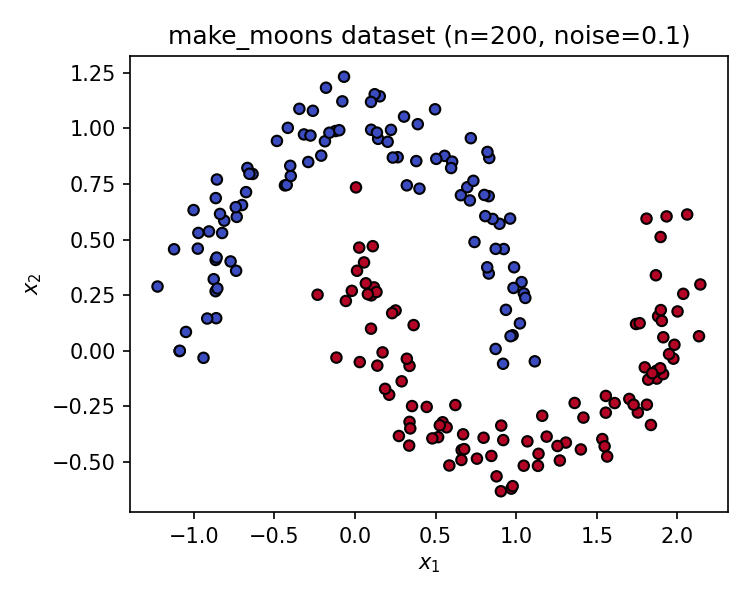
\includegraphics[width=0.36\linewidth]{figures/dataset.png}\hfill
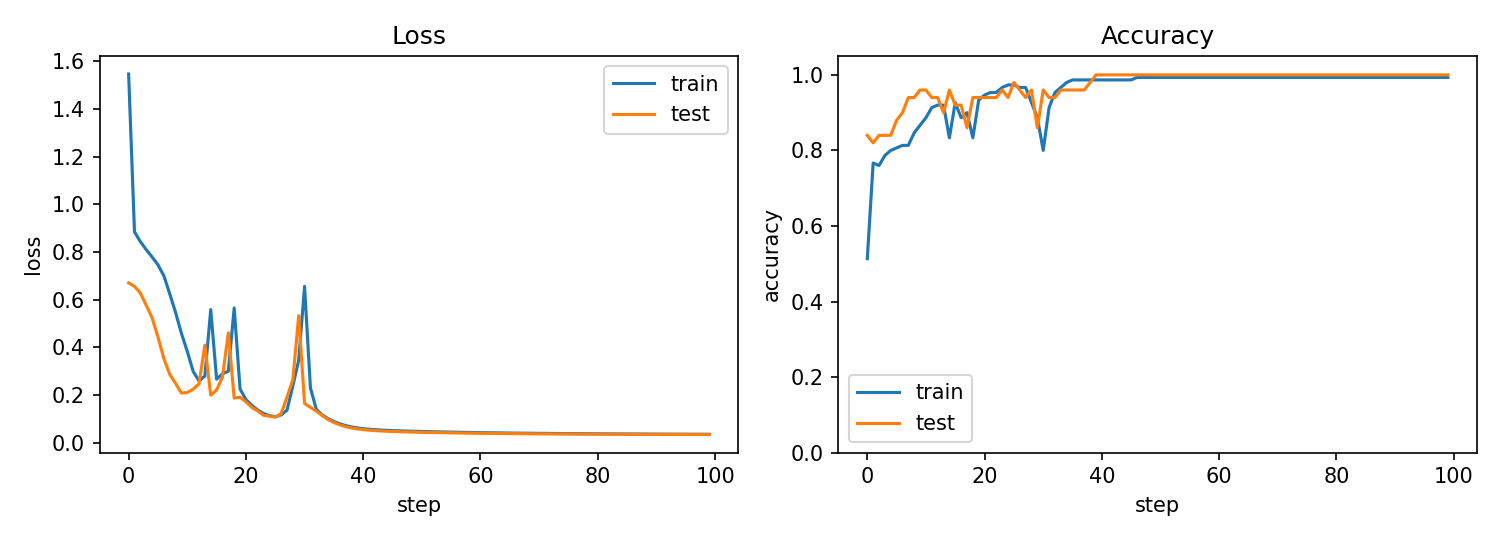
\includegraphics[width=0.6\linewidth]{figures/training_curves.png}
\caption{Left: dataset. Right: loss and accuracy per training step.}
\end{figure}

\begin{center}
\begin{tabular}{lcc}
\toprule
 & Loss & Accuracy \\
\midrule
Step 0 (train) & 1.5459 & 51.3\,\% \\
Final (train, 150 points) & 0.0353 & 99.3\,\% \\
Final (test, 50 points) & 0.0341 & 100.0\,\% \\
\bottomrule
\end{tabular}
\end{center}
Training took about 157\,s on a laptop CPU. Around step 30 the training loss rose temporarily
(0.18 at step 20 to 0.66 at step 30) before converging. This is an overshoot caused by the large early learning rate,
and it disappears as the rate decays. With only 50 test points, 100\,\% test accuracy means the boundary
separates this particular split. It should not be read as a precise error estimate.

\begin{figure}[H]
\centering
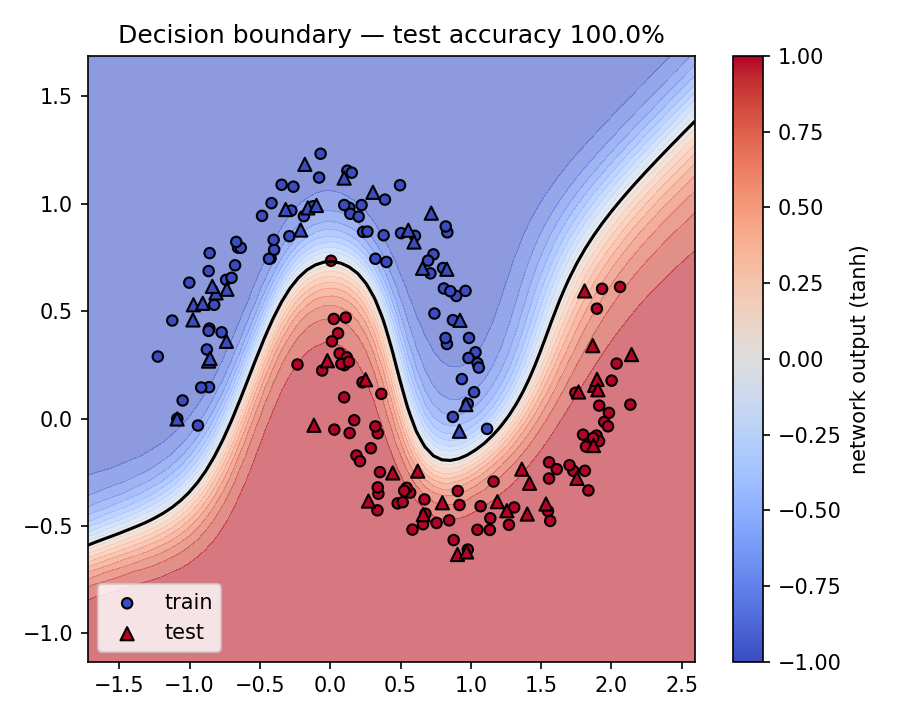
\includegraphics[width=0.55\linewidth]{figures/decision_boundary.png}
\caption{Learned decision boundary (black contour = output 0). Circles: train, triangles: test.}
\end{figure}
\begin{figure}[H]
\centering
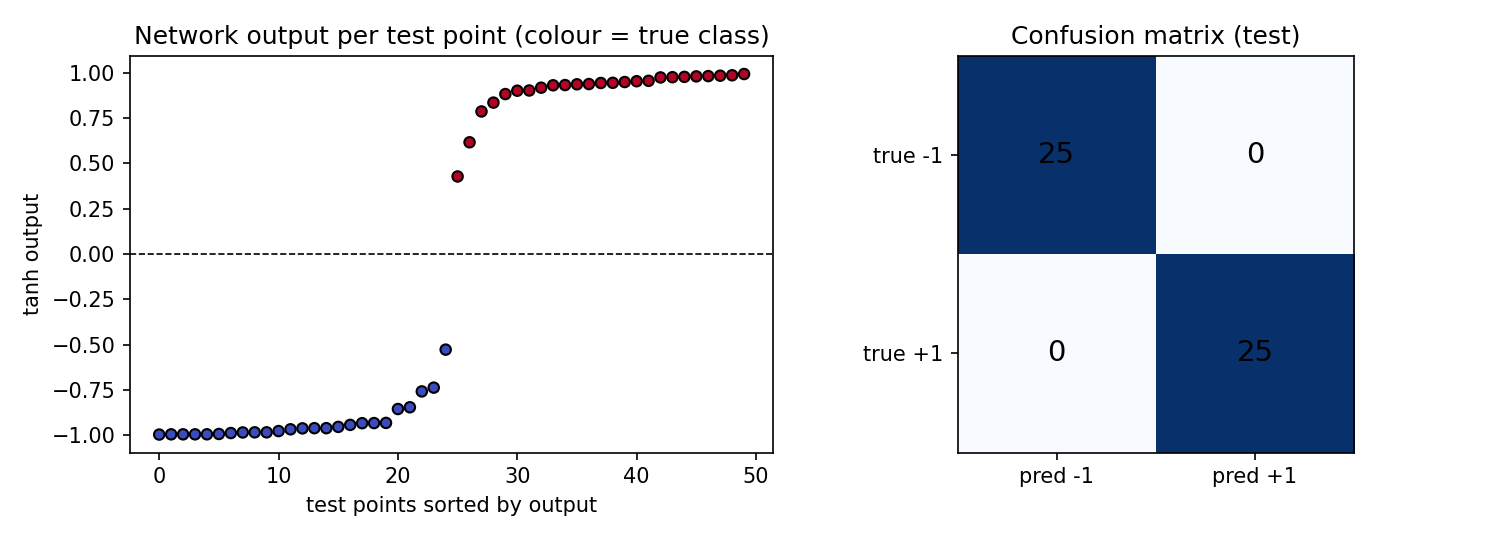
\includegraphics[width=0.9\linewidth]{figures/actual_vs_predicted.png}
\caption{Test-set outputs coloured by true class, and the test confusion matrix (25/25 correct per class).}
\end{figure}

% ================================================================== 15
\section{Design Justifications}
\begin{itemize}
  \item \textbf{Closures for \texttt{\_backward}.} Each node carries exactly the information its derivative needs.
        There is no central table of operations, and adding an operator only means writing one method.
  \item \textbf{Minimal primitive set.} Only $+$, $\times$, power, $\tanh$, $\exp$ have hand-written derivatives.
        Subtraction, negation and division are compositions, so they cannot have inconsistent gradients.
  \item \textbf{\texttt{NotImplemented} for unsupported types} instead of raising directly. Python then tries the reflected
        operator of the other operand and finally raises the standard \texttt{TypeError}, which is the idiomatic protocol.
  \item \textbf{\texttt{assert} in \texttt{\_\_pow\_\_}} as required by the template. A \texttt{Value} exponent would need the
        derivative $a^n\ln a$ with respect to $n$, which is out of scope.
  \item \textbf{Accumulating gradients} (\texttt{+=}, no automatic reset) for correctness on shared nodes and to match the
        PyTorch convention, with explicit \texttt{zero\_grad()}.
  \item \textbf{Recursive DFS} exactly as specified. It is simple and $O(V+E)$. Its limitation (recursion depth) is documented above.
  \item \textbf{Template API preserved}: all class and method signatures are unchanged, so the official autograder runs as-is.
        The only additions are \texttt{\_\_rsub\_\_}, \texttt{\_\_rtruediv\_\_} (so \texttt{1 - x} and \texttt{1 / x} work),
        the \texttt{\_wrap} helper and the input checks in \texttt{Neuron}.
\end{itemize}

% ================================================================== 16
\section{Conclusion}
We implemented a complete scalar reverse-mode automatic differentiation engine and a small neural-network
library on top of it. The engine builds the computational graph through operator overloading, attaches the
local derivative of each operation as a closure, orders the graph with a post-order DFS, and backpropagates
by applying the chain rule in reverse topological order with accumulated gradients. All 12 official tests
and 30 additional tests pass, and analytic gradients agree with finite differences to about $10^{-10}$.
Using only this engine, an MLP trained by gradient descent learns the non-linear two-moons boundary
(99.3\,\% train, 100\,\% test accuracy). The main limitation is speed: one Python object per scalar.
Frameworks such as PyTorch apply the same algorithm to tensors.

\end{document}
